\documentclass[a4paper,12pt]{book}
\usepackage[utf8]{inputenc}
\title{}
\author{Rachel Morris}
\date{\today}

\usepackage{rachwidgets}
\usepackage{fancyhdr}
\usepackage{lastpage}
\usepackage{boxedminipage}

\pagestyle{fancy}
\fancyhf{}
\lhead{CS 250}
\chead{Fall 2017}
\rhead{Lab 3: Static Array Wrapper}
\rfoot{\thepage\ of \pageref{LastPage}}
\lfoot{By Rachel Morris, \footnotesize last updated \today}

\renewcommand{\headrulewidth}{2pt}
\renewcommand{\footrulewidth}{1pt}

\begin{document}

    \chapter*{Lab 3: Static Array Wrapper} \stepcounter{chapter}

        \section*{Information}
            \paragraph{ Topics: } Static arrays, basic data structure functionality, unit tests
            \paragraph{ Turn in: } All source files (.cpp and .hpp).


% ----------------------------------------------------------------------
% ----------------------------------------------------------------------
% ----------------------------------------------------------------------
        \section*{Getting started}

            Make sure to download the starter code for this project.
            It contains quite a few files. You will need to create
            a project and add each of them in.

            
\begin{framed}
\dirtree{%
.1 Lab 3 - Static Array Wrapper/.
.2 lab3\_SmartStaticArray{.}hpp.
.2 lab3\_SmartStaticArray{.}cpp.
.2 lab3\_main{.}cpp.
.2 lab3\_tester{.}hpp.
.3 cuTEST/.
.4 Menu.hpp.
.4 StringUtil.hpp.
.4 TesterBase.hpp.
.4 TesterBase.cpp.
}    
\end{framed}

            The items under the \textbf{cuTEST} folder is a unit test
            library that I've written, and is needed in order to use
            the \texttt{lab3\_tester.hpp} file. When you run the program
            you will be able to test one function of your SmartStaticArray
            at a time.

            \newpage
            In Code::Blocks, the project directory will look like this: ~\\

            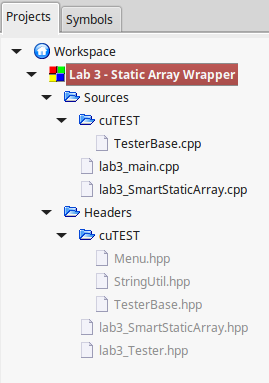
\includegraphics{images/lab3_projecttree.png}

            \begin{intro}{Need help setting up the project?}
                There are helper documents on my Course Common Files repository on GitHub,
                https://github.com/Rachels-Courses/Course-Common-Files

                ~\\
                Go to STUDENT\_REFERENCE $\to$ HOW\_TO, where you will find
                helper docs on using Code Blocks and Visual Studio.
            \end{intro}
        
            \paragraph{WHY ALL THESE FILES?! O\_O} ~\\
            You will only be implementing the SmartStaticArray class' functions,
            but I've gone ahead and created the program shell.

            All this program does is start up and being the tests, and
            the tests run all the functions in the SmartStaticArray class,
            whose declarations and definitions are included in
            \texttt{lab3\_SmartStaticArray.hpp} and \\
            \texttt{lab3\_SmartStaticArray.cpp}.

            ~\\
            My cuTEST library also contains some other reusable code,
            such as \texttt{Menu.hpp}, which contains functions to make
            ``pretty" console menus, and \texttt{StringUtil.hpp},
            which contains my functions to convert between numbers
            and strings.

            \paragraph{What are unit tests?} ~\\
            Unit tests are a type of tests that test one \textit{unit}
            at a time - usually a single function in a program. The
            idea behind unit tests is that, for any given function,
            we know what the \textbf{expected outputs} are for some
            \textbf{given inputs}. We can then run the function
            with those inputs, and compare the \textbf{actual output}
            to the expected output.

            You don't need to know how the unit test code in this assignment
            works, but we will go over writing unit tests later on in class.

            ~\\
            When you run the program, you will have a main menu where you
            can choose which function to test:

\begin{lstlisting}[style=output]
--------------------------------------------------------------------------------
- cuTEST Main Menu -
--------------------------------------------------------------------------------
1. Push
2. Insert
3. Extend
4. Pop
5. Remove
6. Get
7. Size
8. IsFull
9. IsEmpty
10. operator[]
11. operator=
12. operator==
13. Exit

Enter choice (1 - 13): 
\end{lstlisting}

            ~\\
            When you run a test, it will give you an error message if
            a test fails. This will help you figure out if your function
            is working correctly, and help protect against logic errors.

\begin{lstlisting}[style=output]
--------------------------------------------------------------------------------
- TestPop() -
--------------------------------------------------------------------------------
TEST FAILED: TestPop() A
Tried to pop from an empty array. New list size is negative!

TEST FAILED: TestPop() B
Array's size after pushing MAX_SIZE items is not MAX_SIZE.

TEST FAILED: TestPop() C
Popped all items from an array. IsEmpty is false, but should be true.
\end{lstlisting}

            It will also give you a summary of how many tests passed,
            so you will be able to see that you're progressing as you go.

            \begin{error}{Warning!}
                It is very important to make sure your program compiles
                and runs at all times! If you keep trying to implement
                all the functions while the program is not in a building
                state, you cannot take advantage of the unit tests!
                
                ~\\
                The best way to approach this is to work on
                \textbf{one function at a time}, or even part of one
                function at a time, and build after every few changes.

                ~\\
                Points are taken off for turning in code that doesn't build.
            \end{error}

\newpage
\section*{The SmartStaticArray class declaration}

        The class declaration for the SmartStaticArray has already been
        written, and looks like this:

\begin{lstlisting}[style=code]
const int MAX_SIZE = 1000;

class SmartStaticArray
{
    public:
    SmartStaticArray();

    void Push( const string& newItem );
    void Insert( int index, const string& newItem );
    void Extend( const SmartStaticArray& other );
    void Pop();
    void Remove( int index );
    string Get( int index ) const;

    int Size() const;
    bool IsFull() const;
    bool IsEmpty() const;

    string operator[]( int index );
    SmartStaticArray& operator=( const SmartStaticArray& other );
    bool operator==( const SmartStaticArray& other );
    bool operator!=( const SmartStaticArray& other );

    private:
    void ShiftRight( int index );
    void ShiftLeft( int index );

    string m_data[MAX_SIZE];
    int m_itemCount;
};
\end{lstlisting}

        ~\\
        Take note of the private member variables,
        \texttt{m\_data} and \texttt{m\_itemCount},
        which will be used within the function definitions.

\newpage
\section*{Implementing the functions}

        Step through the instructions on how to implement each of these functions.
        
        ~\\
        Note that, for certain tests, certain functions need to be implemented
        for the tests to work correctly. For example, the \texttt{Pop()} function
        test won't work properly until the \texttt{Push()} function has
        been implemented as well.


    \subsection*{SmartStaticArray()}

    \begin{framed} ~\\
        \textbf{Input parameters:} None \\
        \textbf{Return value:} None
    \end{framed}

    In this constructor function, you only need to initialize the
    private member variable, \texttt{m\_itemCount}, to 0.

    % ---------------------------------------------------------------- %
    \hrulefill
    \subsection*{int Size()}

    \begin{framed} ~\\
        \textbf{Input parameters:} None \\
        \textbf{Return value:} int, the amount of items stored in the array.
    \end{framed}

    This function will only return the current value of the
    private member variable, \texttt{m\_itemCount}.
    
    % ---------------------------------------------------------------- %
    \hrulefill
    \subsection*{bool IsFull()}

    \begin{framed} ~\\
        \textbf{Input parameters:} None \\
        \textbf{Return value:} bool, true if the array is full, or false if it is not.
    \end{framed}

    You can determine whether the array is full by comparing \texttt{m\_itemCount}
    with \texttt{MAX\_SIZE}. If they are equivalent, then the array is full.
    
    % ---------------------------------------------------------------- %
    \hrulefill
    \subsection*{bool IsEmpty()}

    \begin{framed} ~\\
        \textbf{Input parameters:} None \\
        \textbf{Return value:} bool, true if the array is empty, or false if it is not.
    \end{framed}

    You can determine whether the array is full by checking if \texttt{m\_itemCount}
    's value is 0. If it is 0, then the array is empty.

    \begin{hint}{Hint: Shortcut!}
        While you could write an if/else statement for this and the \texttt{IsFull()}
        functions, you can also simply do...:

\begin{verbatim}
bool SmartStaticArray::IsEmpty() const
{
    return ( m_itemCount == 0 );
}
\end{verbatim}

        ... which will return true if \texttt{( m\_itemCount == 0 )},
        and false if not.
    \end{hint}
    
    % ---------------------------------------------------------------- %
    \hrulefill
    \subsection*{string Get( int index )}

    \begin{framed} ~\\
        \textbf{Input parameters:} int index \\
        \textbf{Return value:} string, the value from the array
    \end{framed}

    \paragraph{Error checking:} Make sure to check if the index is valid
    before trying to access the array! The index is invalid if it is
    less than 0, or greater than or equal to the \texttt{m\_itemCount}.

    If the index is invalid, \textbf{throw} an \texttt{out\_of\_range}
    error with a message: ``Cannot get at index - out of range".

    \paragraph{Functionality:} If the index is valid, then this function
    will return the value from the private member array, \texttt{m\_data},
    at the position passed in as \texttt{index}.
    
    % ---------------------------------------------------------------- %
    \hrulefill
    \subsection*{void Pop()}

    \begin{framed} ~\\
        \textbf{Input parameters:} None \\
        \textbf{Return value:} None
    \end{framed}

    The Pop() function is used to remove the very last item of the array.
    However, we are going to do something called a \textbf{lazy delete}:
    we don't \textit{actually} have to change any data; we can simply adjust
    the \texttt{m\_itemCount} variable to say that there is one less item.

    Therefore, in this function, first check to make sure that \texttt{m\_itemCount}
    is greater than 0. If so, then simply decrement \texttt{m\_itemCount} by one.

    \begin{hint}{Decrementing variables}
        There are several ways you can decrement a variable:
\begin{verbatim}
1. num = num - 1;
2. num -= 1;
3. num--;
4. --num;
\end{verbatim}
    \end{hint}
    
    % ---------------------------------------------------------------- %
    \hrulefill
    \subsection*{void ShiftRight( int index )}

    \begin{framed} ~\\
        \textbf{Input parameters:} int index, the location to begin pushing items forward \\
        \textbf{Return value:} None \\
        \textbf{Specifier:} This function won't throw an exception. Mark it as \texttt{noexcept}.
    \end{framed}

    For this function, we are going to shift all the items in the array
    to the right one space. This is so that we can make space for a new
    item when the \texttt{Insert} function is called.

    ~\\
    Create a for loop:
    \begin{itemize}
        \item Start: Create a counter variable \texttt{i} and initialize it to
            \texttt{m\_itemCount}.
        \item Loop condition: While \texttt{i} is greater than the \texttt{index}.
        \item Update code: Decrement \texttt{i} by 1 each time.
    \end{itemize}

    Within the loop, set the value of \texttt{m\_data} at position \texttt{i}
    to the value of \texttt{m\_data} at position \texttt{i-1}.

    \begin{hint}{English $\to$ Code}
        Since we're early on in the class, and you might be a bit rusty
        at C++, here's what this function is supposed to look like!

\begin{verbatim}
void SmartStaticArray::ShiftRight( int index )
{
    for ( int i = m_itemCount; i > index; i-- )
    {
        m_data[i] = m_data[i-1];
    }
}
\end{verbatim}
    \end{hint}
    
    % ---------------------------------------------------------------- %
    \hrulefill
    \subsection*{void ShiftLeft( int index )}

    \begin{framed} ~\\
        \textbf{Input parameters:} int index, the location to begin pulling items backwards \\
        \textbf{Return value:} None \\
        \textbf{Specifier:} This function won't throw an exception. Mark it as \texttt{noexcept}.
    \end{framed}

    When removing an item at a specific index, we will need to close the
    gap left over; we want all the data in the array to be contiguous.
    Therefore, we need a ShiftLeft function, that will move all the elements
    after a certain index back by one. To implement this...
    
    ~\\
    Create a for loop:
    \begin{itemize}
        \item Start: Create a counter variable \texttt{i} and initialize it to the \texttt{index}.
        \item Loop condition: While \texttt{i} is less than \texttt{m\_itemCount - 1}.
        \item Update code: Increment \texttt{i} by 1 each time.
    \end{itemize}

    Within the loop, set the value of \texttt{m\_data} at position \texttt{i}
    to the value of \texttt{m\_data} at position \texttt{i+1}.
    
    % ---------------------------------------------------------------- %
    \hrulefill
    \subsection*{void Push( const string\& newItem )}

    \begin{framed} ~\\
        \textbf{Input parameters:} const string\& newItem \\
        \textbf{Return value:} None
    \end{framed}

    \paragraph{Error checking:} Make sure to check if the array is full
    before we add any new items, otherwise we will go outside of bounds of the array!

    Create an if statement that asks if the array is full (you can use the
    \texttt{IsFull()} function. If the array is full, then
    \textbf{throw} a \texttt{length\_error}
    error with a message: ``Cannot add new item - array is full!".

    \paragraph{Functionality:} If the array is not full, then you will
    add the \texttt{newItem} to the array \texttt{m\_data}, at the
    position \texttt{m\_itemCount}. Also make sure to increment
    \texttt{m\_itemCount} by one afterwards.

    \begin{hint}{Storing the new value}
        \begin{verbatim} m_data[ m_itemCount ] = newItem; \end{verbatim}
    \end{hint}
    
    
    % ---------------------------------------------------------------- %
    \hrulefill
    \subsection*{void Insert( int index, const string\& newItem )}

    \begin{framed} ~\\
        \textbf{Input parameters:} int index, const string\& newItem \\
        \textbf{Return value:} None
    \end{framed}

    \paragraph{Error checking:} For this function, there are several
    things we want to check for before we make any modifications to the array.
    Make sure to check for...

    \begin{itemize}
        \item If the index is invalid (less than 0, or greater than or equal to \texttt{MAX\_SIZE}). ~\\
        If the index is invalid, then \textbf{throw} an \texttt{out\_of\_range}
        exception with the message, ``Cannot insert at index - out of range".
        
        \item If the array is full (use \texttt{IsFull()}. ~\\
        If the array is full, then \textbf{throw} a \texttt{length\_error}
        exception with the message, ``Cannot insert new item - array is full!".
        
        \item If the index given is not contiguous in the array. ~\\
        If the index is in a bad position, then \textbf{throw} an \texttt{out\_of\_range}
        exception with the message, ``Cannot insert at index - must be contiugous!"
    \end{itemize}
    
    \paragraph{Functionality:}
    If everything is OK (no exceptions are thrown), then...

    \begin{enumerate}
        \item Call the \texttt{ShiftRight} function, passing in the index.
        \item Assign the value \texttt{newItem} to the element of \texttt{m\_data}
            at the given index.
        \item Increment \texttt{m\_itemCount} by one.
    \end{enumerate}


    
    % ---------------------------------------------------------------- %
    \hrulefill
    \subsection*{void Extend( const SmartStaticArray\& other )}

    \begin{framed} ~\\
        \textbf{Input parameters:} const SmartStaticArray\& other \\
        \textbf{Return value:} None
    \end{framed}

    This function takes a second SmartStaticArray as its input parameter.
    The values from the other SmartStaticArray will be appended to the
    end of the array we're working with from within this function.
    
    \paragraph{Error checking:}
    Check to see if the sum of \texttt{m\_itemCount} and
    \texttt{other.m\_itemCount} is greater than or equal to \texttt{MAX\_SIZE}.
    If it is greater, then \textbf{throw} a \texttt{length\_error} with
    the message, ``Cannot append second list - will go out of bounds of array!"

    \paragraph{Functionality:}
    If there is no error, then you will create a for loop to iterate
    through all the items from the \texttt{other} SmartStaticArray,
    and add them to our current SmartStaticArray via the \texttt{Push} function.

    \begin{hint}{Hint: Copying over the values}
\begin{verbatim}
for ( int i = 0; i < other.m_itemCount; i++ )
{
    Push( other.Get( i ) );
}
\end{verbatim}
    \end{hint}
    
    
    % ---------------------------------------------------------------- %
    \hrulefill
    \subsection*{void Remove( int index )}

    \begin{framed} ~\\
        \textbf{Input parameters:} None \\
        \textbf{Return value:} None
    \end{framed}

    \paragraph{Error checking:}
    Check to see if the index is invalid (less than 0 or greater than
    or equal to \texttt{m\_itemCount}). If it is invalid, then
    \textbf{throw} an \texttt{out\_of\_range} exception
    with the message, ``Cannot insert at index - out of range".
    
    \paragraph{Functionality:}
    If there is no exception thrown, then call the \texttt{ShiftLeft}
    function, passing in the index. Again, we are \textit{lazy deleting}
    the data by simply overwriting it with this function call.

    Afterwards, make sure to decrement \texttt{m\_itemCount}.
    
    % ---------------------------------------------------------------- %
    \hrulefill
    \subsection*{Remaining functions}

    There are several functions that are \textbf{overloaded operators},
    which are already implemented for you:
    \texttt{operator=}, \texttt{operator==}, and \texttt{operator!=}.

    \hrulefill{}
    \subsection*{Running and testing}

    Make sure your program compiles and runs. Test out each function
    one at a time via the tester menu.

    It is best to make sure that your program runs after every change
    you make, so that you can use the unit tests to check your work
    as you're going through.

    \newpage

\chapter*{}

\section*{Grading breakdown}

\begin{tabular}{ | p{8cm} | p{4cm} | }
    \hline
    \textbf{Function} & \textbf{Point value}
    \\ \hline
    
    SmartStaticArray constructor & 1       \\ \hline
    Size & 1       \\ \hline
    IsFull & 1       \\ \hline
    IsEmpty & 1       \\ \hline
    Get & 2       \\ \hline
    Pop & 2       \\ \hline
    ShiftRight & 3       \\ \hline
    ShiftLeft & 3       \\ \hline
    Push & 3       \\ \hline
    Insert & 5       \\ \hline
    Extend & 5       \\ \hline
    Remove & 3       \\ \hline
    & \\ \hline
    \textbf{Total} & 30
    \\ \hline    
\end{tabular}

\newpage
\section*{Appendix A: Starter code}

\subsection*{lab3\_main.cpp}

\begin{lstlisting}[style=code]
#include <iostream>
using namespace std;

#include "lab3_Tester.hpp"

int main()
{
    Tester tester;
    tester.Start();

    return 0;
}  
\end{lstlisting}

\subsection*{lab3\_SmartStaticArray.hpp}

\begin{lstlisting}[style=code]
#ifndef _SMART_STATIC_ARRAY_HPP
#define _SMART_STATIC_ARRAY_HPP

#include <iostream>
#include <string>
#include <stdexcept>
using namespace std;

const int MAX_SIZE = 1000;

class SmartStaticArray
{
    public:
    SmartStaticArray();

    void Push( const string& newItem );
    void Insert( int index, const string& newItem );
    void Extend( const SmartStaticArray& other );
    void Pop();
    void Remove( int index );
    string Get( int index ) const;

    int Size() const;
    bool IsFull() const;
    bool IsEmpty() const;

    string operator[]( int index );
    SmartStaticArray& operator=( const SmartStaticArray& other );
    bool operator==( const SmartStaticArray& other );
    bool operator!=( const SmartStaticArray& other );

    private:
    void ShiftRight( int index );
    void ShiftLeft( int index );

    string m_data[MAX_SIZE];
    int m_itemCount;
};

#endif
\end{lstlisting}

\subsection*{lab3\_SmartStaticArray.hpp}

\begin{lstlisting}[style=code]
#include "lab3_SmartStaticArray.hpp"

#include "cuTEST/Menu.hpp"

SmartStaticArray::SmartStaticArray()
{
}

int SmartStaticArray::Size() const
{
        return -1; // placeholder
}

bool SmartStaticArray::IsFull() const
{
        return false; // placeholder
}

bool SmartStaticArray::IsEmpty() const
{
        return false; // placeholder
}

string SmartStaticArray::Get( int index ) const
{
    return ""; // placeholder
}

void SmartStaticArray::Pop()
{
}

void SmartStaticArray::ShiftRight( int index )
{
}

void SmartStaticArray::ShiftLeft( int index )
{
}

void SmartStaticArray::Push( const string& newItem )
{
}

void SmartStaticArray::Insert( int index, const string& newItem )
{
}

void SmartStaticArray::Extend( const SmartStaticArray& other )
{
}

void SmartStaticArray::Remove( int index )
{
}

SmartStaticArray& SmartStaticArray::operator=( const SmartStaticArray& other )
{
        for ( int i = 0; i < other.m_itemCount; i++ )
        {
        m_data[i] = other.m_data[i];
        m_itemCount++;
        }

        return *this;
}

bool SmartStaticArray::operator==( const SmartStaticArray& other )
{
        if ( m_itemCount != other.m_itemCount )
        {
        return false;
        }

        for ( int i = 0; i < m_itemCount; i++ )
        {
        if ( m_data[i] != other.m_data[i] )
        {
            return false;
        }
        }

        return true;
}

bool SmartStaticArray::operator!=( const SmartStaticArray& other )
{
        return !( *this == other );
}

string SmartStaticArray::operator[]( int index )
{
    return Get( index );
}
\end{lstlisting}

\subsection*{Additional files}

There are other files needed for this lab, though you can download them
from the class GitHub page.

\end{document}









